\chapter{न्यूक्लियोटाइड और न्यूक्लिक अम्ल}\label{ch:b1:nucleic-acids}

टूटी हुई \omterm{def:b1:cell-unit-of-life:cell}{कोशिकाओं} के किसी विलयन पर ठंडा एथेनॉल उँड़ेलिए और तंतुओं का एक
सफ़ेद बादल उभर आता है जिसे किसी काँच की छड़ पर लपेटा जा सकता है: \omterm{def:b1:nucleic-acids:chain}{DNA},
यानी वह अणु जो \omterm{def:b1:organism-environment:organism}{जीव} का हर निर्देश ढोता है, नंगी आँख से दिखता हुआ। हर मानव
केंद्रक में उसके दो मीटर मुड़े हुए हैं; और वह सारा का सारा चार अक्षरों की
वर्णमाला में लिखा है, एक ही दिशा में पढ़ा जाता है, और दो ऐसी लड़ियों को
अलग करके नक़ल किया जाता है जो एक-दूसरे में हाथ और दस्ताने की तरह बैठती
हैं। यह अध्याय \omterm{def:b1:nucleic-acids:nucleotide}{न्यूक्लियोटाइडों} का --- जो एक ही साथ अक्षर, ऊर्जा-मुद्रा
और सहएंजाइम हैं --- उनकी बनाई शृंखलाओं का, द्विकुंडली और उसके साक्ष्य का,
उसके पिघलने और फिर जुड़ने पर क्या होता है इसका, और उन \omterm{def:b1:nucleic-acids:chain}{RNA} का वर्णन करता
है जो उसका संदेश \omterm{def:b1:cell-unit-of-life:cell}{कोशिका} तक ले जाते हैं।

\section{न्यूक्लियोटाइड}

\begin{definition}[न्यूक्लियोटाइड]\label{def:b1:nucleic-acids:nucleotide}
कोई \emph{न्यूक्लियोटाइड}\index{न्यूक्लियोटाइड} तीन भागों का बना है: एक
नाइट्रोजनी \emph{क्षारक}\index{नाइट्रोजनी क्षारक} --- कोई
\emph{प्यूरीन}\index{प्यूरीन} (ऐडेनीन A, ग्वानीन G: दो संगलित वलय) या कोई
\emph{पिरिमिडीन}\index{पिरिमिडीन} (साइटोसीन C, थाइमीन T, यूरैसिल U:
एक वलय); पाँच कार्बन की एक शर्करा, \omterm{def:b1:nucleic-acids:chain}{RNA} में \emph{राइबोस} या \omterm{def:b1:nucleic-acids:chain}{DNA} में
\emph{2$'$-डिऑक्सीराइबोस} (जिसमें कार्बन $2'$ पर हाइड्रॉक्सिल
नहीं होता); और शर्करा के कार्बन $5'$ पर एक से तीन तक \emph{फ़ॉस्फ़ेट}
समूह। क्षारक कार्बन $1'$ से जुड़ता है; और शर्करा के कार्बनों को
क्षारक के कार्बनों से अलग दिखाने के लिए अंकों पर प्राइम लगाया जाता है।
क्षारक और शर्करा मिलकर कोई \emph{न्यूक्लियोसाइड} (ऐडेनोसिन, ग्वानोसिन,
साइटिडीन, थाइमिडीन, यूरिडीन) हैं; और फ़ॉस्फ़ेटों के साथ वह
न्यूक्लियोटाइड (AMP, ADP, \omterm{def:b1:water-small-molecules:atp}{ATP} और उनके सजातीय)।
\end{definition}

\begin{omfigure}
\begin{tikzpicture}[font=\footnotesize, line cap=round, line join=round]
  % phosphates
  \foreach \i/\c in {0/omThm!15,1/omThm!25,2/omThm!35} {
    \draw[thick, omThm!80!black, fill=\c, rounded corners=3pt] (1.3*\i,0.9) rectangle (1.3*\i+1.1,1.9);
    \node at (1.3*\i+0.55,1.4) {$\mathrm{P}$};
  }
  \node[anchor=south, align=center] at (1.65,2.15) {फ़ॉस्फ़ेट: $\gamma$, $\beta$, $\alpha$\\ (उनके बीच ऐनहाइड्राइड बंध)};
  \draw[thick] (3.3,1.4) -- (4.0,1.4);
  % sugar pentagon
  \draw[thick, omDef!80!black, fill=omDef!15] (4.0,1.4) -- (4.55,2.05) -- (5.45,2.05) -- (6.0,1.4) -- (5.0,0.85) -- cycle;
  \node at (5.0,1.5) {राइबोस};
  \node[font=\scriptsize] at (3.85,1.15) {$5'$};
  \node[font=\scriptsize] at (4.55,2.25) {$4'$};
  \node[font=\scriptsize] at (5.45,2.25) {$1'$};
  \node[font=\scriptsize] at (6.15,1.15) {$2'$};
  \node[font=\scriptsize] at (5.0,0.6) {$3'$};
  \draw[thick] (5.0,0.85) -- (5.0,0.2) node[below] {OH};
  \draw[thick] (6.0,1.4) -- (6.6,1.0) node[right] {OH (डिऑक्सीराइबोस में H)};
  % base
  \draw[thick] (5.45,2.05) -- (5.9,2.7);
  \draw[thick, omExo!80!black, fill=omExo!15, rounded corners=3pt] (5.4,2.7) rectangle (7.6,3.7);
  \node at (6.5,3.2) {क्षारक (A, G, C, U/T)};
  \node[anchor=west, align=left, gray] at (8.2,3.0) {न्यूक्लियोसाइड = क्षारक + शर्करा\\ न्यूक्लियोटाइड = न्यूक्लियोसाइड + फ़ॉस्फ़ेट\\ ATP = ऐडेनीन + राइबोस + तीन फ़ॉस्फ़ेट};
\end{tikzpicture}

{\small किसी \omterm{def:b1:nucleic-acids:nucleotide}{न्यूक्लियोटाइड} के भाग: किसी पेंटोस के कार्बन $1'$ पर एक
\omterm{def:b1:nucleic-acids:nucleotide}{क्षारक}, और कार्बन $5'$ पर फ़ॉस्फ़ेट। $3'$ हाइड्रॉक्सिल वह जगह है जहाँ
शृंखला का अगला \omterm{def:b1:nucleic-acids:nucleotide}{न्यूक्लियोटाइड} जुड़ेगा; और $2'$ स्थान \omterm{def:b1:nucleic-acids:chain}{RNA} (OH) को \omterm{def:b1:nucleic-acids:chain}{DNA} (H)
से अलग करता है।}
\end{omfigure}

\begin{proposition}[न्यूक्लियोटाइड तीन काम करते हैं]\label{prop:b1:nucleic-acids:threejobs}
\omterm{def:b1:nucleic-acids:chain}{DNA} और \omterm{def:b1:nucleic-acids:chain}{RNA} के एकलक होने के अलावा \omterm{def:b1:nucleic-acids:nucleotide}{न्यूक्लियोटाइड} \omterm{def:b1:cell-unit-of-life:cell}{कोशिका} की
\emph{\omterm{def:b1:water-small-molecules:atp}{ऊर्जा मुद्रा}} हैं --- \omterm{def:b1:water-small-molecules:atp}{ATP} और GTP, जिनके \omterm{def:b1:water-small-molecules:atp}{फ़ॉस्फ़ोऐनहाइड्राइड बंध}
(\cref{ch:b1:water-small-molecules}) संश्लेषण, अभिगमन और गति की क़ीमत
चुकाते हैं; उसके \emph{सहएंजाइम} --- $\mathrm{NAD^+}$, $\mathrm{NADP^+}$
और FAD, जो श्वसन तथा प्रकाश-संश्लेषण में इलेक्ट्रॉन ढोते हैं
(\cref{ch:b1:respiration-fermentation}), और सहएंजाइम A, जो ऐसिल समूह
ढोता है; और उसके \emph{संदेशवाहक} --- चक्रीय AMP, जो \omterm{def:b1:cell-unit-of-life:cell}{कोशिकाओं} के भीतर
हॉर्मोन के संकेत पहुँचाता है। ये सब ऐडेनीन \omterm{def:b1:nucleic-acids:nucleotide}{न्यूक्लियोटाइड} हैं या उन्हीं
पर बने हैं: जो अणु संदेश लिखता है वही उसके निष्पादन को शक्ति भी देता है।
\end{proposition}

\section{बहुन्यूक्लियोटाइड शृंखला}

\begin{definition}[फ़ॉस्फ़ोडाइएस्टर बंध, ध्रुवता]\label{def:b1:nucleic-acids:chain}
\omterm{def:b1:nucleic-acids:nucleotide}{न्यूक्लियोटाइड} \emph{फ़ॉस्फ़ोडाइएस्टर बंधों}\index{फ़ॉस्फ़ोडाइएस्टर बंध}
से किसी \emph{बहुन्यूक्लियोटाइड}\index{बहुन्यूक्लियोटाइड} में जुड़ते
हैं: किसी एक \omterm{def:b1:nucleic-acids:nucleotide}{न्यूक्लियोटाइड} के कार्बन $5'$ का फ़ॉस्फ़ेट अगले के $3'$
हाइड्रॉक्सिल से जुड़ता है। इसलिए शृंखला की एक शर्करा--फ़ॉस्फ़ेट
\emph{रीढ़} होती है, जो एकसमान और ऋण-आवेशित है (प्रति फ़ॉस्फ़ेट एक
आवेश), और जिससे \omterm{def:b1:nucleic-acids:nucleotide}{क्षारक} एक अनुक्रम के रूप में बाहर निकले रहते हैं; और उसकी
एक दिशा होती है: एक \emph{$5'$ सिरा}\index{5' end@$5'$ सिरा} जो मुक्त
फ़ॉस्फ़ेट धारण करता है और एक \emph{$3'$ सिरा}\index{3' end@$3'$ सिरा} जो
मुक्त हाइड्रॉक्सिल। अनुक्रम $5' \to 3'$ लिखे और पढ़े जाते हैं, यानी उसी
दिशा में जिसमें शृंखलाएँ संश्लेषित होती हैं। \emph{DNA}\index{DNA}
(डिऑक्सीराइबोन्यूक्लिक अम्ल) डिऑक्सीराइबोस और \omterm{def:b1:nucleic-acids:nucleotide}{क्षारक} A, G, C, T काम में
लेता है; \emph{RNA}\index{RNA} (राइबोन्यूक्लिक अम्ल) राइबोस और A, G, C, U।
\end{definition}

\begin{omfigure}
\begin{tikzpicture}[font=\footnotesize, line cap=round]
  \foreach \i/\b in {0/A,1/C,2/G,3/T} {
    \draw[thick, omThm!80!black, fill=omThm!25, rounded corners=2pt] (0.3,-1.6*\i+0.15) rectangle (0.9,-1.6*\i+0.75);
    \node at (0.6,-1.6*\i+0.45) {P};
    \draw[thick, omDef!80!black, fill=omDef!15] (1.3,-1.6*\i-0.1) -- (1.6,-1.6*\i+0.3) -- (2.2,-1.6*\i+0.3) -- (2.5,-1.6*\i-0.1) -- (1.9,-1.6*\i-0.5) -- cycle;
    \node[font=\scriptsize] at (1.9,-1.6*\i-0.1) {शर्करा};
    \draw[thick] (0.9,-1.6*\i+0.45) -- (1.3,-1.6*\i-0.1);
    \node[font=\scriptsize] at (1.2,-1.6*\i+0.4) {$5'$};
    \node[font=\scriptsize] at (2.0,-1.6*\i-0.75) {$3'$};
    \draw[thick] (2.2,-1.6*\i+0.3) -- (2.9,-1.6*\i+0.3);
    \draw[thick, omExo!80!black, fill=omExo!15, rounded corners=2pt] (2.9,-1.6*\i+0.0) rectangle (3.7,-1.6*\i+0.6);
    \node at (3.3,-1.6*\i+0.3) {\b};
  }
  \foreach \i in {0,1,2} { \draw[thick] (1.9,-1.6*\i-0.5) -- (0.6,-1.6*\i-0.85); }
  \node[anchor=east, align=right] at (0.1,0.9) {$5'$ सिरा:\\ मुक्त फ़ॉस्फ़ेट};
  \node[anchor=east, align=right] at (0.1,-5.5) {$3'$ सिरा:\\ मुक्त हाइड्रॉक्सिल};
  \draw[thick] (1.9,-5.3) -- (1.9,-5.7) node[below, font=\scriptsize] {OH};
  \draw[->, very thick, gray] (4.6,0.6) -- (4.6,-5.2) node[midway, right, align=left] {$5' \to 3'$ पढ़ा\\ और लिखा जाता है:\\ यह लड़ी\\ $5'$-ACGT-$3'$ है};
  \draw[thick, omThm!80!black] (0.4,-0.9) -- (0.4,-1.3);
  \node[anchor=west, align=left, gray] at (7.4,-2.6) {रीढ़: एकांतर शर्करा\\ और फ़ॉस्फ़ेट, प्रति फ़ॉस्फ़ेट\\ एक ऋण आवेश\\ क्षारक: परिवर्ती भाग,\\ यानी अनुक्रम};
\end{tikzpicture}

{\small चार \omterm{def:b1:nucleic-acids:nucleotide}{न्यूक्लियोटाइडों} की एक शृंखला। हर \omterm{def:b1:nucleic-acids:nucleotide}{न्यूक्लियोटाइड} का $5'$
फ़ॉस्फ़ेट ऊपर वाले के $3'$ हाइड्रॉक्सिल से किसी \omterm{def:b1:nucleic-acids:chain}{फ़ॉस्फ़ोडाइएस्टर बंध} से
जुड़ा है; शृंखला किसी $5'$ सिरे से किसी $3'$ सिरे तक चलती है और \omterm{def:b1:nucleic-acids:nucleotide}{क्षारक}
एक एकसमान रीढ़ से लटके रहते हैं।}
\end{omfigure}

\begin{example}[RNA नाज़ुक है, DNA टिकाऊ]\label{ex:b1:nucleic-acids:fragile}
राइबोस का $2'$ हाइड्रॉक्सिल पड़ोसी \omterm{def:b1:nucleic-acids:chain}{फ़ॉस्फ़ोडाइएस्टर बंध} पर हमला कर सकता
है: हल्के क्षार में \omterm{def:b1:nucleic-acids:chain}{RNA} घंटों के भीतर जल-अपघटित होकर \omterm{def:b1:nucleic-acids:nucleotide}{न्यूक्लियोटाइड} बन
जाता है, जबकि \omterm{def:b1:nucleic-acids:chain}{DNA}, जिसमें वह हाइड्रॉक्सिल नहीं है, क्षार में उबाल सह लेता
है और दसियों हज़ार वर्ष पुरानी हड्डियों से साबुत निकाला जा चुका है। \omterm{def:b1:nucleic-acids:chain}{RNA}
का यूरैसिल बिना मेथिल समूह का थाइमीन है; \omterm{def:b1:nucleic-acids:chain}{DNA} थाइमीन इसलिए काम में लेता है
कि साइटोसीन, जो धीरे-धीरे अपना ऐमीनो समूह खोकर यूरैसिल बन जाता है, क्षति
के रूप में पहचाना और मरम्मत किया जा सके --- \omterm{def:b1:nucleic-acids:chain}{DNA} में कोई यूरैसिल सदा एक
भूल है।
\end{example}

\section{द्विकुंडली}

\begin{proposition}[चारगाफ़ के नियम]\label{prop:b1:nucleic-acids:chargaff}
\index{चारगाफ़ के नियम}
किसी भी \omterm{def:b1:organism-environment:organism}{जीव} के \omterm{def:b1:nucleic-acids:chain}{DNA} में ऐडेनीन की मात्रा थाइमीन की मात्रा के बराबर होती
है और ग्वानीन की मात्रा साइटोसीन की ($A = T$,
$G = C$, इसलिए \omterm{def:b1:nucleic-acids:nucleotide}{प्यूरीन} $=$ \omterm{def:b1:nucleic-acids:nucleotide}{पिरिमिडीन}), जबकि अनुपात $(G + C)/(A + T)$
जाति-दर-जाति बदलता है (\qty{25}{\%} से \qty{75}{\%}
$G + C$ तक)।
\end{proposition}
\begin{proof}[साक्ष्य]
चारगाफ़ (1950) ने अनेक \omterm{def:b1:organism-environment:organism}{जीवों} का \omterm{def:b1:nucleic-acids:chain}{DNA} जल-अपघटित किया और क्षारकों को
वर्णलेखन से अलग किया, हर एक को उसके पराबैंगनी अवशोषण से मापते हुए।
हर \omterm{def:b1:nucleic-acids:chain}{DNA} के लिए ये समानताएँ प्रायोगिक त्रुटि के भीतर टिकीं;
$G + C$ की मात्रा नहीं टिकी, और वह किसी एक \omterm{def:b1:organism-environment:organism}{जीव} के हर \omterm{def:b1:body-plans-tissues:tissue}{ऊतक} में एक ही थी।
\end{proof}

\begin{theorem}[वॉटसन--क्रिक द्विकुंडली]\label{thm:b1:nucleic-acids:helix}
\index{द्विकुंडली}\index{क्षारक युग्म}\index{प्रतिसमांतर}
\omterm{def:b1:nucleic-acids:chain}{DNA} दो \omterm{def:b1:nucleic-acids:chain}{बहुन्यूक्लियोटाइड} शृंखलाएँ हैं जो किसी साझा अक्ष के चारों ओर एक
दक्षिणावर्त \emph{द्विकुंडली} में लिपटी हैं: शर्करा--फ़ॉस्फ़ेट रीढ़ें
बाहर, और \omterm{def:b1:nucleic-acids:nucleotide}{क्षारक} भीतर, चपटे और अक्ष के लंब चिने हुए।
शृंखलाएँ \emph{प्रतिसमांतर} हैं (एक ऊपर की ओर $5' \to 3'$ चलती है और
दूसरी नीचे की ओर) और \emph{पूरक}: हर A के सामने एक T है, जो दो \omterm{def:b1:water-small-molecules:water}{हाइड्रोजन
बंधों} से थमा है, और हर G के सामने एक C, जो तीन से; और ऐसा हर
\emph{\omterm{thm:b1:nucleic-acids:helix}{क्षारक युग्म}} एक ही चौड़ाई का है, इसलिए अनुक्रम कोई भी हो, कुंडली
एकसमान रहती है। आम B रूप में कुंडली \qty{2}{nm} चौड़ी है, प्रति \omterm{thm:b1:nucleic-acids:helix}{क्षारक
युग्म} \qty{0.34}{nm} और दस युग्मों के प्रति फेरे \qty{3.4}{nm} चढ़ती है,
और एक चौड़ी \emph{मुख्य खाँच} तथा एक सँकरी \emph{गौण खाँच} दिखाती है,
जिनमें क्षारकों के किनारे प्रोटीनों के सामने खुले रहते हैं।
\end{theorem}
\begin{proof}[साक्ष्य]
फ़्रैंकलिन के \omterm{def:b1:nucleic-acids:chain}{DNA} तंतुओं के X-किरण विवर्तन चित्रों (1952) ने किसी कुंडली
का क्रॉस दिखाया, जिसकी अक्ष के सहारे पुनरावृत्ति \qty{3.4}{nm} थी, एक
प्रबल परावर्तन \qty{0.34}{nm} पर (चिनी हुई चपटी इकाइयाँ), और व्यास
\qty{2}{nm}; और फ़ॉस्फ़ेटों को, जो सबसे भारी परमाणु हैं, बाहर होना ही
था। वॉटसन और क्रिक (1953) ने पाया कि किसी \omterm{def:b1:nucleic-acids:nucleotide}{प्यूरीन} का किसी
\omterm{def:b1:nucleic-acids:nucleotide}{पिरिमिडीन} से युग्म --- और वह भी केवल A का T से और G का C से --- बराबर
चौड़ाई के ऐसे युग्म देता है जो \qty{2}{nm} व्यास में बैठते हैं और जो
\omterm{prop:b1:nucleic-acids:chargaff}{चारगाफ़ के नियम} समझा देते हैं, और यह भी कि इस तरह युग्मित दो प्रतिसमांतर
शृंखलाएँ उस तंतु की मापों वाली एक नियमित कुंडली बनाती हैं। मॉडल ने
भविष्यवाणी की कि हर शृंखला दूसरी के लिए साँचा है; और मेसेल्सन तथा स्टाल
के अर्ध-संरक्षी प्रतिकृतिकरण के प्रदर्शन (जो लाइसेयी खंड से याद है,
और \cref{ch:b1:replication-mitosis} में है) ने उसकी पुष्टि की।
\end{proof}

\begin{omfigure}
\begin{minipage}[b]{0.34\linewidth}\centering
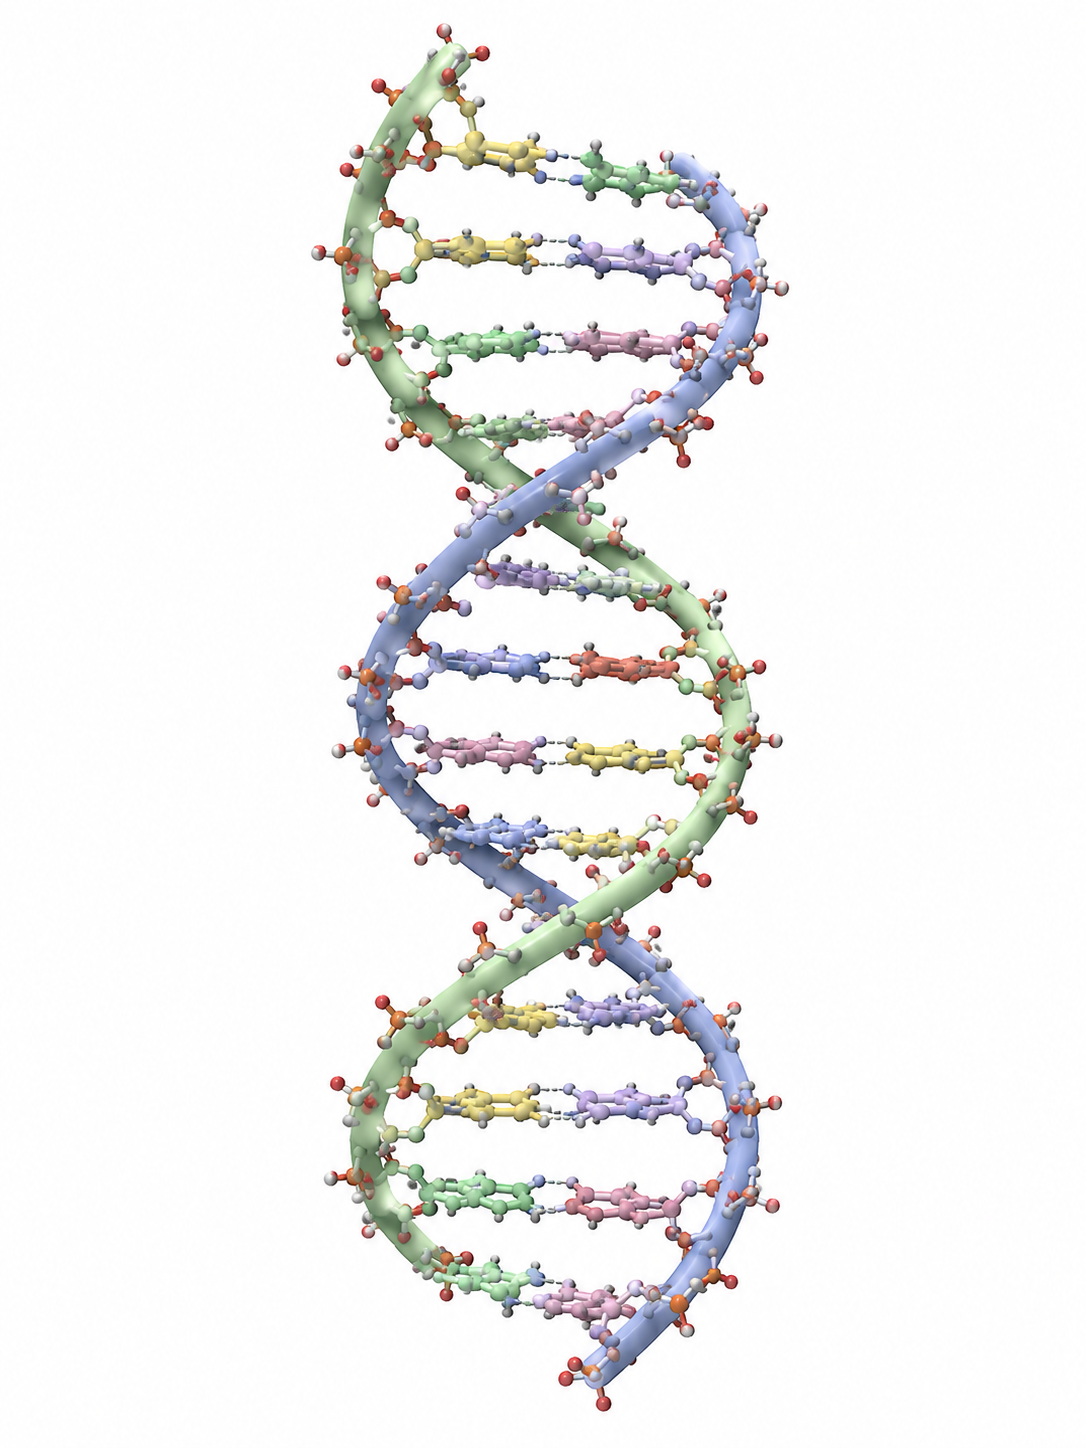
\includegraphics[width=0.9\linewidth]{images/book3/ai/fig-dna-double-helix.png}
\end{minipage}\hfill
\begin{minipage}[b]{0.62\linewidth}\centering
\begin{tikzpicture}[font=\footnotesize, line cap=round]
  % two antiparallel backbones as vertical bars, base pairs as rungs
  \draw[line width=3pt, omDef] (0,0) -- (0,5.1);
  \draw[line width=3pt, omDef!50] (2.6,0) -- (2.6,5.1);
  \foreach \i/\l/\r/\n in {0/A/T/2,1/G/C/3,2/T/A/2,3/C/G/3,4/A/T/2,5/G/C/3,6/C/G/3,7/T/A/2,8/G/C/3,9/A/T/2} {
    \pgfmathsetmacro{\y}{0.3+0.5*\i}
    \draw[thick, omExo!80!black, fill=omExo!20] (0.1,\y-0.14) rectangle (1.2,\y+0.14);
    \draw[thick, omExo!80!black, fill=omExo!20] (1.4,\y-0.14) rectangle (2.5,\y+0.14);
    \node[font=\scriptsize] at (0.65,\y) {\l}; \node[font=\scriptsize] at (1.95,\y) {\r};
    \ifnum\n=3 \draw[dashed] (1.2,\y-0.08) -- (1.4,\y-0.08) (1.2,\y) -- (1.4,\y) (1.2,\y+0.08) -- (1.4,\y+0.08);
    \else \draw[dashed] (1.2,\y-0.05) -- (1.4,\y-0.05) (1.2,\y+0.05) -- (1.4,\y+0.05); \fi
  }
  \node[anchor=south, omDef] at (0,5.15) {$5'$}; \node[anchor=north, omDef] at (0,-0.05) {$3'$};
  \node[anchor=south, omDef!70!black] at (2.6,5.15) {$3'$}; \node[anchor=north, omDef!70!black] at (2.6,-0.05) {$5'$};
  \draw[<->, thick] (3.2,0.3) -- (3.2,4.8) node[midway, right, align=left] {दस क्षारक युग्म\\ $= \qty{3.4}{nm}$\\ $=$ एक फेरा};
  \draw[<->, thick] (3.2,-0.6) -- (3.2,0.3) node[midway, right] {};
  \draw[<->, thick] (0,-0.9) -- (2.6,-0.9) node[midway, below] {\qty{2}{nm}};
  \draw[<->, thick] (-0.5,0.3) -- (-0.5,0.8) node[midway, left] {\qty{0.34}{nm}};
  \node[anchor=west, align=left, font=\scriptsize] at (3.2,5.2) {A--T पर 2 हाइड्रोजन बंध\\ G--C पर 3 हाइड्रोजन बंध};
\end{tikzpicture}
\end{minipage}

{\small बाएँ: द्विकुंडली का एक मॉडल; दोनों रीढ़ें चिने हुए \omterm{thm:b1:nucleic-acids:helix}{क्षारक युग्मों}
के चारों ओर लिपटती हैं और एक मुख्य तथा एक गौण खाँच छोड़ती हैं।
दाएँ: वही दस \omterm{thm:b1:nucleic-acids:helix}{क्षारक युग्म} खोलकर एक सीढ़ी के रूप में: प्रतिसमांतर
लड़ियाँ, बराबर चौड़ाई के पूरक युग्म, प्रति युग्म \qty{0.34}{nm}
और प्रति फेरा \qty{3.4}{nm}।}
\end{omfigure}

\begin{example}[किसी लड़ी को पढ़ना]\label{ex:b1:nucleic-acids:complement}
यदि एक लड़ी $5'$-ATGGCATTC-$3'$ पढ़ी जाए, तो उसकी साथी, जिसे
$5' \to 3'$ लिखा जाता है, $5'$-GAATGCCAT-$3'$ है: हर \omterm{def:b1:nucleic-acids:nucleotide}{क्षारक} का पूरक
लीजिए, फिर क्रम उलट दीजिए। नौ युग्म, \qty{3.1}{nm} कुंडली, बाईस
\omterm{def:b1:water-small-molecules:water}{हाइड्रोजन बंध} (पाँच G--C, चार A--T)। \num{2.5e8} युग्मों का कोई मानव
गुणसूत्र इस रूप में \qty{8.5}{cm} लंबा है और किसी केंद्रक में समाने के
लिए उसे एक लाख गुना मुड़ना पड़ता है (\cref{ch:b1:genomes})।
\end{example}

\begin{proposition}[कुंडली को क्या थामे रखता है]\label{prop:b1:nucleic-acids:stability}
युग्मित क्षारकों के बीच के \omterm{def:b1:water-small-molecules:water}{हाइड्रोजन बंध} विशिष्टता देते हैं; चपटे
क्षारकों का एक-दूसरे पर \emph{स्तरण}\index{क्षारक-स्तरण}
--- यानी \omterm{def:b1:water-small-molecules:bonds}{वान डर वाल्स} संपर्क और वह \omterm{prop:b1:water-small-molecules:properties}{जलविरागी प्रभाव} जो क्षारकों को जल से
बाहर रखता है --- अधिकांश स्थायित्व देता है; ऋण-आवेशित रीढ़ें एक-दूसरे को
प्रतिकर्षित करती हैं, और कुंडली केवल तभी स्थायी है जब ऐसे धनायन उपस्थित
हों (शरीरक्रियात्मक $\mathrm{Mg^{2+}}$, $\mathrm{Na^+}$, या क्रोमैटिन के
क्षारीय प्रोटीन) जो उस आवेश को परिरक्षित कर दें। तीन \omterm{def:b1:water-small-molecules:water}{हाइड्रोजन बंधों} और
अधिक प्रबल \omterm{prop:b1:nucleic-acids:stability}{स्तरण} वाला कोई G--C युग्म किसी A--T युग्म से बेहतर थामता है।
\end{proposition}

\section{पिघलना और संकरण}

\begin{definition}[विकृतीकरण, गलन ताप]\label{def:b1:nucleic-acids:melting}
ऊष्मा, या चरम pH, \omterm{def:b1:nucleic-acids:chain}{DNA} की दोनों लड़ियाँ अलग कर देती है:
\emph{विकृतीकरण}\index{विकृतीकरण (DNA)} (पिघलना), यानी कुछ ही डिग्री पर
होता एक सहकारी संक्रमण, जिसका मध्यबिंदु \emph{गलन
ताप}\index{गलन ताप} $T_m$ है। उसके साथ
\emph{अतिवर्णी प्रभाव} आता है: एकल लड़ियाँ \qty{260}{nm} पर उन्हीं
क्षारकों से लगभग \qty{40}{\%} अधिक पराबैंगनी प्रकाश अवशोषित करती हैं जो
किसी कुंडली में चिने हों। $T_m$ $G + C$ की मात्रा के साथ बढ़ता है
(प्रति प्रतिशत \qty{0.4}{\celsius}), लवण की सांद्रता के साथ, और लंबाई के
साथ; \qty{0.15}{mol/L} लवण में \qty{50}{\%} $G + C$ का कोई लंबा \omterm{def:b1:nucleic-acids:chain}{DNA}
\qty{90}{\celsius} के पास पिघलता है। धीरे-धीरे ठंडा करने पर लड़ियाँ अपने
पूरक ढूँढ़ लेती हैं और कुंडली फिर बना लेती हैं: \emph{पुनर्प्राकृतिकरण},
या \emph{संकरण}\index{संकरण} जब लड़ियाँ अलग-अलग स्रोतों से आई हों।
\end{definition}

\begin{omfigure}
\begin{tikzpicture}
\begin{axis}[
  width=0.86\linewidth, height=6.0cm,
  axis x line=bottom, axis y line=left,
  xmin=60, xmax=105, ymin=0.95, ymax=1.5,
  xlabel={ताप (\unit{\celsius})}, ylabel={\qty{260}{nm} पर सापेक्ष अवशोषकता},
  xlabel style={font=\small, at={(axis description cs:0.5,-0.12)}, anchor=north},
  ylabel style={font=\small},
  tick label style={font=\small}, xtick={60,70,80,90,100}, ytick={1.0,1.2,1.4},
  legend style={font=\small, at={(0.03,0.97)}, anchor=north west, draw=none},
  clip=false,
]
\addplot[very thick, omDef, domain=60:105, samples=120] {1+0.4/(1+exp(-(x-77)/1.5))};
\addlegendentry{\qty{30}{\%} $G+C$: $T_m = \qty{77}{\celsius}$}
\addplot[very thick, omThm, domain=60:105, samples=120] {1+0.4/(1+exp(-(x-93)/1.5))};
\addlegendentry{\qty{70}{\%} $G+C$: $T_m = \qty{93}{\celsius}$}
\draw[dashed, gray] (axis cs:60,1.2) -- (axis cs:93,1.2);
\draw[dashed, gray] (axis cs:77,0.95) -- (axis cs:77,1.2);
\draw[dashed, gray] (axis cs:93,0.95) -- (axis cs:93,1.2);
\end{axis}
\end{tikzpicture}

{\small एक ही लवण में दो \omterm{def:b1:nucleic-acids:chain}{DNA} के गलन वक्र। लड़ियों के अलग होते जाने पर
अवशोषकता कुछ ही डिग्री में \qty{40}{\%} बढ़ जाती है; और G--C युग्मों से
अधिक समृद्ध \omterm{def:b1:nucleic-acids:chain}{DNA} के लिए मध्यबिंदु $T_m$ ऊँचा है।}
\end{omfigure}

\begin{method}[अवशोषकता से न्यूक्लिक अम्लों का मापन]\label{met:b1:nucleic-acids:absorbance}
\begin{enumerate}
  \item \omterm{def:b1:nucleic-acids:nucleotide}{क्षारक} पराबैंगनी प्रकाश अवशोषित करते हैं और उनका अधिकतम
        \qty{260}{nm} पर है। \qty{1}{cm} की किसी सेल में $1.0$ की
        अवशोषकता द्विलड़ी \omterm{def:b1:nucleic-acids:chain}{DNA} के \qty{50}{\micro g/mL} के बराबर है
        (\omterm{def:b1:nucleic-acids:chain}{RNA} के \qty{40}{\micro g/mL}, एकलड़ी \omterm{def:b1:nucleic-acids:chain}{DNA} के
        \qty{33}{\micro g/mL})।
  \item अनुपात $A_{260}/A_{280}$ शुद्ध \omterm{def:b1:nucleic-acids:chain}{DNA} के लिए $1.8$ और शुद्ध \omterm{def:b1:nucleic-acids:chain}{RNA} के
        लिए $2.0$ है; प्रोटीन \qty{280}{nm} पर अवशोषित करते हैं और उसे
        घटा देते हैं।
  \item पिघलने का पीछा करने के लिए धीरे-धीरे गरम करते हुए $A_{260}$
        अभिलिखित कीजिए; वक्र का मध्यबिंदु $T_m$ है और उसका ढाल नमूने की
        समांगता का माप।
  \item किसी अनुक्रम को पकड़ने के लिए नमूने को विकृत कीजिए और उसकी पूरक
        कोई चिह्नित एकल लड़ी मिलाइए (कोई \emph{प्रोब}); वह केवल वहीं
        संकरित होती है जहाँ उसका पूरक है, और चिह्न वह जगह बता देता है
        --- किसी जेल पर, किसी गुणसूत्र पर, किसी \omterm{def:b1:body-plans-tissues:tissue}{ऊतक} में।
\end{enumerate}
\end{method}

\begin{omfigure}
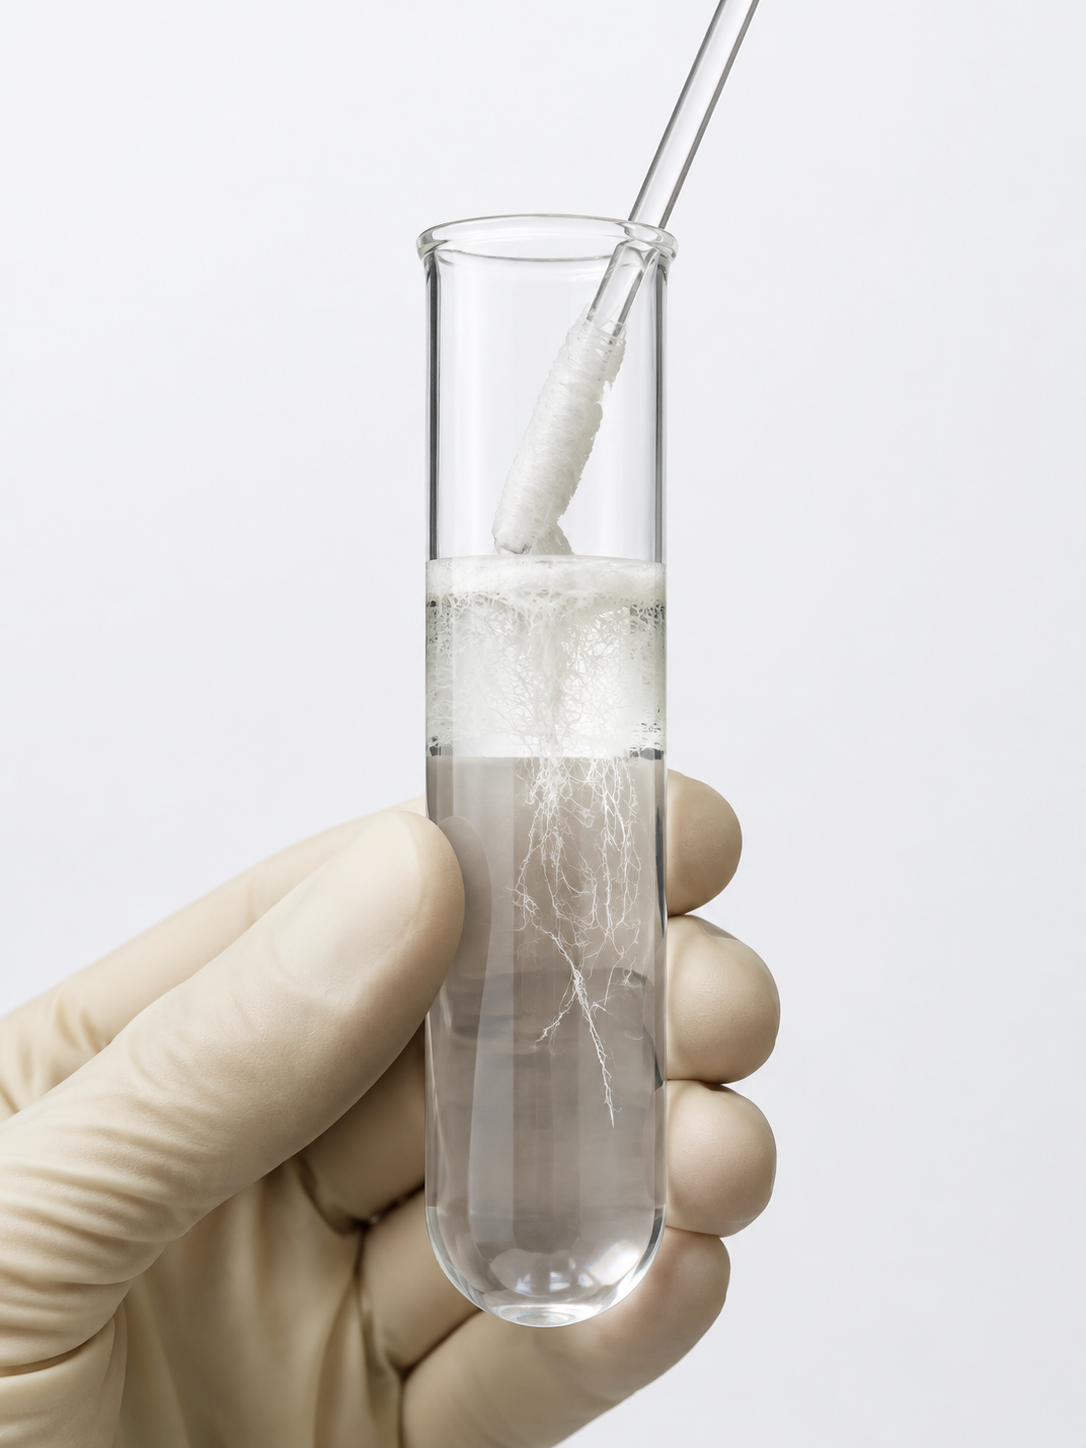
\includegraphics[width=0.3\linewidth]{images/book3/ai/b3-11-dna-precipitate.png}

{\small किसी कोशिका-लयनक से ठंडे एथेनॉल द्वारा अवक्षेपित और काँच की छड़
पर लपेटा गया \omterm{def:b1:nucleic-acids:chain}{DNA}: उस अणु के कुछ मिलीग्राम, जो तंतुओं के रूप में इसलिए
दिखते हैं कि हर अणु लाखों \omterm{thm:b1:nucleic-acids:helix}{क्षारक युग्म} लंबा है।}
\end{omfigure}

\begin{example}[कोई प्रोब किसी जीन को खोज लेता है]\label{ex:b1:nucleic-acids:probe}
किसी एक जीन की पूरक बीस \omterm{def:b1:nucleic-acids:nucleotide}{न्यूक्लियोटाइडों} की कोई प्रोब, अपने ही $T_m$ से
\qty{5}{\celsius} नीचे, तीन अरब \omterm{thm:b1:nucleic-acids:helix}{क्षारक युग्मों} में अपना ठीक पूरक बाँधती
है और कुछ नहीं: बीस में एक भी बेमेल $T_m$ को कई डिग्री गिरा देता है और
बेमेल संकर पिघल जाता है। बीस स्थानों पर गुणित क्षारक-युग्मन की यही
विशिष्टता वह चीज़ है जिस पर पितृत्व से लेकर रोगजनक-पहचान तक हर \omterm{def:b1:nucleic-acids:chain}{DNA} जाँच
टिकी है।
\end{example}

\section{RNA}

\begin{definition}[RNA के प्रकार]\label{def:b1:nucleic-acids:rnas}
\omterm{def:b1:nucleic-acids:chain}{RNA} प्रायः एकलड़ी होता है, और जहाँ कहीं छोटे पूरक खंड अनुमति दें वहाँ
अपने ही ऊपर मुड़कर हेयरपिन, फंदे और उभार बना लेता है
--- यानी एक \emph{द्वितीयक संरचना} --- जो फिर किसी आकृति में जम जाती है।
तीन वर्ग आनुवंशिक जानकारी का प्रवाह ढोते हैं
(\cref{ch:b1:gene-expression}): \emph{संदेशवाहक RNA}\index{संदेशवाहक RNA} (mRNA), जो किसी जीन की वह प्रति है जिसे राइबोसोम पढ़ता है;
\emph{अंतरण RNA}\index{अंतरण RNA} (tRNA), जो कोई \qty{75}{}
\omterm{def:b1:nucleic-acids:nucleotide}{न्यूक्लियोटाइड} हैं और तिपतिया पत्ती में मुड़े रहते हैं, अपने $3'$ सिरे पर
एक ऐमीनो अम्ल ढोते हैं और एक \emph{प्रतिकोडॉन} रखते हैं जो संदेश से
युग्म बनाता है; और \emph{राइबोसोमी RNA}\index{राइबोसोमी RNA} (rRNA), जो
राइबोसोम का संरचनात्मक तथा उत्प्रेरक अंतर्भाग है और किसी \omterm{def:b1:cell-unit-of-life:cell}{कोशिका} के \omterm{def:b1:nucleic-acids:chain}{RNA} का
चार-पाँचवाँ भाग। और भी अनेक \omterm{def:b1:nucleic-acids:chain}{RNA} नियमन, संबंधन तथा पथ-प्रदर्शन करते हैं
(वर्ष 3 का खंड)।
\end{definition}

\begin{omfigure}
\begin{tikzpicture}[font=\footnotesize, line cap=round, >=Stealth]
  % acceptor stem (vertical, top)
  \draw[line width=2.5pt, omDef] (0,0) -- (0,2.2);
  \draw[line width=2.5pt, omDef] (0.5,0) -- (0.5,2.2);
  \foreach \y in {0.3,0.65,1.0,1.35,1.7} { \draw[thick, omExo!80!black] (0,\y) -- (0.5,\y); }
  \node[anchor=south] at (0,2.25) {$5'$};
  \draw[line width=2.5pt, omDef] (0.5,2.2) -- (0.5,2.9) -- (1.0,3.2);
  \node[anchor=west] at (1.0,3.2) {$3'$-CCA: ऐमीनो अम्ल यहाँ जुड़ता है};
  % D arm (left)
  \draw[line width=2.5pt, omDef] (0,0) -- (-1.4,0) (0,-0.5) -- (-1.4,-0.5);
  \foreach \x in {-0.3,-0.65,-1.0} { \draw[thick, omExo!80!black] (\x,0) -- (\x,-0.5); }
  \draw[line width=2.5pt, omDef] (-1.4,0) arc (90:270:0.25);
  \node[anchor=east, align=right] at (-1.8,-0.25) {D भुजा};
  % T arm (right)
  \draw[line width=2.5pt, omDef] (0.5,0) -- (1.9,0) (0.5,-0.5) -- (1.9,-0.5);
  \foreach \x in {0.8,1.15,1.5} { \draw[thick, omExo!80!black] (\x,0) -- (\x,-0.5); }
  \draw[line width=2.5pt, omDef] (1.9,0) arc (90:-90:0.25);
  \node[anchor=west, align=left] at (2.3,-0.25) {T भुजा};
  % anticodon stem (down)
  \draw[line width=2.5pt, omDef] (0,-0.5) -- (0,-2.2) (0.5,-0.5) -- (0.5,-2.2);
  \foreach \y in {-0.85,-1.2,-1.55,-1.9} { \draw[thick, omExo!80!black] (0,\y) -- (0.5,\y); }
  \draw[line width=2.5pt, omDef] (0,-2.2) arc (180:360:0.25);
  \foreach \x in {0.1,0.25,0.4} { \fill[omThm] (\x,-2.5) circle (0.06); }
  \node[anchor=north, align=center] at (0.25,-2.65) {प्रतिकोडॉन फंदा: तीन क्षारक\\ जो mRNA के किसी कोडॉन से युग्म बनाते हैं};
  \node[anchor=west, align=left, gray] at (2.3,1.2) {युग्मित क्षारकों के चार तने\\ (तिपतिया पत्ती), जो त्रिविम में\\ मुड़कर एक L बनते हैं};
\end{tikzpicture}

{\small अपनी तिपतिया-पत्ती द्वितीयक संरचना में एक \omterm{def:b1:nucleic-acids:rnas}{अंतरण RNA}: लगभग 75
\omterm{def:b1:nucleic-acids:nucleotide}{न्यूक्लियोटाइडों} की एक ही लड़ी, जो अपने ही साथ युग्मित होकर चार \omterm{def:b1:flowering-plant-organization:organs}{तने} बनाती
है। ऐमीनो अम्ल $3'$ सिरे पर ढोया जाता है; और सामने वाले सिरे का
प्रतिकोडॉन संदेश पढ़ता है।}
\end{omfigure}

\begin{remark}[RNA उत्प्रेरक भी हो सकता है]\label{rem:b1:nucleic-acids:ribozyme}
कुछ \omterm{def:b1:nucleic-acids:chain}{RNA} एंजाइम हैं (\emph{राइबोज़ाइम}): हर प्रोटीन का पेप्टाइड बंध
\omterm{def:b1:nucleic-acids:rnas}{राइबोसोमी RNA} बनाता है, कोई प्रोटीन नहीं, और कुछ \omterm{def:b1:nucleic-acids:chain}{RNA} स्वयं को काटते और
जोड़ते हैं। जो अणु एक ही साथ जानकारी ढोता हो और अभिक्रियाएँ उत्प्रेरित
करता हो, उसी से पहला जीवित तंत्र बना हो सकता है; और तब DNA--प्रोटीन का
संसार श्रम-विभाजन का कोई बाद का चरण होगा, जिसके केंद्र में \omterm{def:b1:nucleic-acids:chain}{RNA} बना रहा।
\end{remark}

\section{अभ्यास}

\begin{exercise}[$\star$]\label{exo:b1:nucleic-acids:1}
किसी \omterm{def:b1:nucleic-acids:nucleotide}{न्यूक्लियोटाइड} के तीन भाग बताइए और किसी राइबोन्यूक्लियोटाइड तथा
किसी डिऑक्सीराइबोन्यूक्लियोटाइड के बीच के दो भेद।
\end{exercise}

\begin{exercise}[$\star$]\label{exo:b1:nucleic-acids:2}
$5'$-GGATCCTA-$3'$ की पूरक लड़ी $5' \to 3'$ दिशा में लिखिए,
और उसके \omterm{def:b1:water-small-molecules:water}{हाइड्रोजन बंध} गिनिए।
\end{exercise}

\begin{exercise}[$\star$]\label{exo:b1:nucleic-acids:3}
किसी \omterm{def:b1:nucleic-acids:chain}{DNA} में \qty{22}{\%} ऐडेनीन है। T, G और C के प्रतिशत दीजिए, और
$G + C$ की मात्रा भी।
\end{exercise}

\begin{exercise}[$\star$]\label{exo:b1:nucleic-acids:4}
गलन वाले आलेख से बताइए कि उन्हीं परिस्थितियों में किसी ऐसे \omterm{def:b1:nucleic-acids:chain}{DNA} का $T_m$
क्या है जिसमें \qty{50}{\%} $G + C$ हो, और पिघलने पर अवशोषकता कितनी
बढ़ती है।
\end{exercise}

\begin{exercise}[$\star\star$]\label{exo:b1:nucleic-acids:5}
\emph{E. coli} गुणसूत्र ($\num{4.6e6}$ \omterm{thm:b1:nucleic-acids:helix}{क्षारक युग्म}) की लंबाई
मिलीमीटर में निकालिए, उसके फेरों की संख्या, और वह गुणक भी जितना उसे
\qty{2}{\micro m} की किसी \omterm{def:b1:cell-unit-of-life:cell}{कोशिका} में समाने के लिए संहत होना पड़ता है।
\end{exercise}

\begin{exercise}[$\star\star$]\label{exo:b1:nucleic-acids:6}
शर्करा--फ़ॉस्फ़ेट रीढ़ की ज्यामिति से और इस आवश्यकता से कि हर \omterm{thm:b1:nucleic-acids:helix}{क्षारक
युग्म} एक ही चौड़ाई का हो, समझाइए कि \omterm{def:b1:nucleic-acids:chain}{DNA} की दोनों लड़ियों को प्रतिसमांतर
क्यों होना चाहिए।
\end{exercise}

\begin{exercise}[$\star\star$]\label{exo:b1:nucleic-acids:7}
\omterm{def:b1:nucleic-acids:chain}{DNA} के किसी विलयन का \qty{1}{cm} सेल में $A_{260} = 0.35$ और
$A_{280} = 0.20$ है। सांद्रता निकालिए और शुद्धता पर टिप्पणी कीजिए।
यदि किसी युग्म का माध्य द्रव्यमान \qty{650}{Da} हो तो \qty{1}{mL} में
कितने \omterm{thm:b1:nucleic-acids:helix}{क्षारक युग्म} हैं?
\end{exercise}

\begin{exercise}[$\star\star$]\label{exo:b1:nucleic-acids:8}
अतिवर्णी प्रभाव समझाइए और यह भी कि किसी शुद्ध \omterm{def:b1:nucleic-acids:chain}{DNA} का गलन वक्र तीखा क्यों
होता है जबकि अनेक जातियों के \omterm{def:b1:nucleic-acids:chain}{DNA} के मिश्रण का वक्र फैला हुआ।
\end{exercise}

\begin{exercise}[$\star\star$]\label{exo:b1:nucleic-acids:9}
बीस \omterm{def:b1:nucleic-acids:nucleotide}{न्यूक्लियोटाइडों} की किसी प्रोब का अपने ठीक पूरक के साथ
$T_m = \qty{62}{\celsius}$ है; एक बेमेल $T_m$ को लगभग \qty{5}{\celsius}
गिरा देता है। ठीक अनुक्रम पकड़ने और एकल बेमेलों को छाँटने के लिए \omterm{def:b1:nucleic-acids:melting}{संकरण}
किस ताप पर किया जाना चाहिए? \qty{45}{\celsius} पर क्या होता है?
\end{exercise}

\begin{exercise}[$\star\star\star$]\label{exo:b1:nucleic-acids:10}
\omterm{prop:b1:nucleic-acids:chargaff}{चारगाफ़ के नियम} द्विलड़ी \omterm{def:b1:nucleic-acids:chain}{DNA} के लिए टिकते हैं, पर \omterm{def:b1:nucleic-acids:chain}{RNA} के लिए नहीं और कुछ
छोटे विषाणुओं के \omterm{def:b1:nucleic-acids:chain}{DNA} के लिए भी नहीं। समझाइए कि हर अपवाद उन न्यूक्लिक
अम्लों की संरचना के बारे में क्या बताता है।
\end{exercise}

\begin{exercise}[$\star\star\star$]\label{exo:b1:nucleic-acids:11}
किसी A--T युग्म को दो \omterm{def:b1:water-small-molecules:water}{हाइड्रोजन बंध} थामते हैं, फिर भी एक हज़ार A--T
युग्मों की कोई कुंडली \qty{60}{\celsius} पर स्थायी है जबकि कोई अकेला
युग्म बनता ही नहीं। \cref{ch:b1:water-small-molecules} के विचारों
(दुर्बल बंध, सहकारिता, \omterm{prop:b1:nucleic-acids:stability}{स्तरण}) से समझाइए, और बताइए कि इससे किसी प्रोब की
सत्यनिष्ठा के बारे में क्या निकलता है।
\end{exercise}

\begin{exercise}[$\star\star\star$]\label{exo:b1:nucleic-acids:12}
``\omterm{def:b1:nucleic-acids:chain}{DNA} की संरचना ही आनुवंशिकता की व्याख्या है।'' एक अनुच्छेद में चर्चा
कीजिए: द्विकुंडली तुरंत क्या समझा देती है (नक़ल, अनुक्रम के परिवर्तन के
रूप में उत्परिवर्तन), वह अपने आप क्या नहीं समझाती (अनुक्रम प्रोटीन कैसे
बनता है), और वॉटसन तथा क्रिक का मॉडल किसी जैवरासायनिक जाँच से पहले ही
क्यों स्वीकार कर लिया गया।
\end{exercise}

\section{समस्या: किसी विषाणु का जीनोम}

\begin{problem}[{सप्ताहांत समस्या --- फ़ेज $\lambda$ का DNA मापा,
तौला, गिना, पिघलाया और उसके कैप्सिड में भरा गया, और अंत में उसका गलन ताप
तथा उसकी परिरेखा-लंबाई}]
\label{pb:b1:nucleic-acids:1}
जीवाणुभोजी $\lambda$ का जीनोम \num{48502} \omterm{thm:b1:nucleic-acids:helix}{क्षारक युग्मों} का एक रैखिक
द्विलड़ी \omterm{def:b1:nucleic-acids:chain}{DNA} है जिसकी $G + C$ मात्रा \qty{49.9}{\%} है। वह
\qty{55}{nm} भीतरी व्यास के किसी बीस-फलकी कैप्सिड में भरा है।
प्रति \omterm{thm:b1:nucleic-acids:helix}{क्षारक युग्म} \qty{0.34}{nm}, कुंडली का व्यास \qty{2.0}{nm},
प्रति \omterm{thm:b1:nucleic-acids:helix}{क्षारक युग्म} \qty{650}{Da}, और $T_m = 81.5 + 16.6\log_{10}[\mathrm{Na^+}]
+ 0.41\,(\%\,G{+}C) - 500/L$ डिग्री सेल्सियस में लीजिए, जिसमें
$[\mathrm{Na^+}]$ \unit{mol/L} में है और $L$ लंबाई \omterm{thm:b1:nucleic-acids:helix}{क्षारक युग्मों} में।

\medskip
\noindent\textbf{भाग I --- मापा और तौला गया।}
\begin{enumerate}
  \item अणु की परिरेखा-लंबाई माइक्रोमीटर में निकालिए।
  \item कुंडली के फेरों की संख्या निकालिए।
  \item उसका मोलर द्रव्यमान डाल्टन में निकालिए।
  \item एक अणु का द्रव्यमान ग्राम में निकालिए।
  \item फ़ॉस्फ़ेट समूहों की संख्या और उससे अणु का शुद्ध आवेश निकालिए।
  \item हर \omterm{def:b1:nucleic-acids:nucleotide}{क्षारक} (A, T, G, C) के \omterm{def:b1:nucleic-acids:nucleotide}{न्यूक्लियोटाइडों} की संख्या निकालिए।
  \item दोनों लड़ियों को थामते \omterm{def:b1:water-small-molecules:water}{हाइड्रोजन बंधों} की कुल संख्या निकालिए।
\end{enumerate}

\medskip
\noindent\textbf{भाग II --- पिघलाया गया।}
\begin{enumerate}[resume]
  \item \qty{0.1}{mol/L} सोडियम में $T_m$ निकालिए।
  \item \qty{0.01}{mol/L} सोडियम में $T_m$ निकालिए, और समझाइए कि लवण
        कुंडली को स्थायी क्यों करता है।
  \item $\lambda$ जीनोम में \qty{35}{\%} $G + C$ का \qty{1000}{}
        युग्मों वाला एक क्षेत्र है और \qty{62}{\%} वाला एक। हर क्षेत्र
        का $T_m$ \qty{0.1}{mol/L} सोडियम में निकालिए और पूरे अणु के गलन
        वक्र की आकृति का वर्णन कीजिए।
  \item $\lambda$ \omterm{def:b1:nucleic-acids:chain}{DNA} के किसी विलयन का पिघलने से पहले $A_{260} = 0.50$
        है। उसकी सांद्रता क्या है, और पूरी तरह पिघलने के बाद $A_{260}$
        क्या होगा?
  \item उस विलयन के \qty{1}{mL} में कितने $\lambda$ अणु हैं?
  \item $\lambda$ जीनोम के दोनों सिरे 12 \omterm{def:b1:nucleic-acids:nucleotide}{न्यूक्लियोटाइडों} के एकलड़ी
        उभार हैं, जो एक-दूसरे के पूरक हैं और जिनसे अणु पोषी में
        वृत्ताकार हो जाता है। उनका $T_m$ निकालिए ($L = 12$ लीजिए) और
        बताइए कि फिर भी वह वृत्त \omterm{def:b1:cell-unit-of-life:cell}{कोशिका} के भीतर \qty{37}{\celsius} पर
        क्यों टिका रहता है।
\end{enumerate}

\medskip
\noindent\textbf{भाग III --- भरा गया।}
\begin{enumerate}[resume]
  \item \omterm{def:b1:nucleic-acids:chain}{DNA} का आयतन किसी बेलन के रूप में निकालिए।
  \item कैप्सिड का भीतरी आयतन निकालिए।
  \item \omterm{def:b1:nucleic-acids:chain}{DNA} कैप्सिड का कितना भिन्न भरता है? समांतर बेलनों के सघनतम
        जमाव (\qty{91}{\%}) से तुलना कीजिए।
  \item \omterm{def:b1:nucleic-acids:chain}{DNA} \qty{55}{nm} के किसी गोले में \num{97000} ऋण आवेश ढोता है।
        समझाइए कि \omterm{def:b1:nucleic-acids:chain}{DNA} के साथ कैप्सिड में क्या घुसना चाहिए, और भरा हुआ
        \omterm{def:b1:nucleic-acids:chain}{DNA} खोल पर वह दाब (दसियों वायुमंडल) क्यों लगाता है जो उसे किसी
        जीवाणु में डालने में मदद करता है।
  \item अणु को कैप्सिड की त्रिज्या जितनी त्रिज्या के फंदों में मोड़ना
        पड़ता है। \omterm{def:b1:nucleic-acids:chain}{DNA} लगभग \qty{50}{nm} से कम त्रिज्या पर मुड़ने का
        प्रतिरोध करता है। टिप्पणी कीजिए।
\end{enumerate}

\medskip
\noindent\textbf{भाग IV --- पढ़ा गया।}
\begin{enumerate}[resume]
  \item जीनोम की एक लड़ी $5'$-GGGCGGCGACCT-$3'$ से शुरू होती है। पूरक
        लड़ी $5' \to 3'$ लिखिए।
  \item यदि \num{1200} \omterm{thm:b1:nucleic-acids:helix}{क्षारक युग्मों} का कोई जीन किसी mRNA में अनुलेखित
        हो, तो उस mRNA की लंबाई \omterm{def:b1:nucleic-acids:nucleotide}{न्यूक्लियोटाइडों} में और, प्रति
        \omterm{def:b1:nucleic-acids:nucleotide}{न्यूक्लियोटाइड} \qty{330}{Da} पर, उसका द्रव्यमान क्या होगा?
  \item जीनोम में \num{48502} युग्मों में \qty{75}{} जीन हैं। यदि औसत
        जीन \num{600} युग्मों का हो तो जीनोम का कितना भिन्न कूटलेखी है?
        किसी मानव जीनोम (\qty{1.5}{\%}) से तुलना कीजिए।
  \item जीनोम \qty{37}{\celsius} पर पोषी के एंजाइमों द्वारा
        \qty{20}{min} में प्रतिकृत होता है। यदि प्रतिकृतिकरण एक ही उद्गम
        से शुरू होकर दोनों दिशाओं में चले तो दर \omterm{thm:b1:nucleic-acids:helix}{क्षारक युग्म} प्रति सेकंड
        में निकालिए।
  \item प्रतिकृतिकरण के दौरान दोनों द्विशाखों पर प्रति सेकंड कितने
        \omterm{def:b1:water-small-molecules:water}{हाइड्रोजन बंध} टूटते हैं (प्रश्न 7 का प्रति युग्म माध्य लीजिए)?
  \item कोई उत्परिवर्तन एक G--C युग्म को A--T में बदल देता है। पूरे अणु
        का $T_m$ कितना बदलता है? क्या पिघलने से उसे पकड़ा जा सकता है?
  \item परिणाम बताइए: \qty{0.1}{mol/L} सोडियम में $\lambda$ \omterm{def:b1:nucleic-acids:chain}{DNA} का \omterm{def:b1:nucleic-acids:melting}{गलन
        ताप} और उसकी परिरेखा-लंबाई, तथा वह संहतीकरण जो उसे कैप्सिड में
        बिठा देता है।
\end{enumerate}
\end{problem}
